\section{Mecanismul de asociere}

\begin{frame}{Mecanismul de asociere în sistemul DenseAP}
  \begin{itemize}
    \item DAP-urile active trimit beacon-uri cu SSID ascuns
    \item Fiecare DAP ține un ACL cu MAC-urile clienților
    \item DAP-ul răspunde la Probe Request numai dacă transmițătorul se află în listă
    \item Dacă nu se află în listă, DAP-ul notifică DC
  \end{itemize}
\end{frame}

\begin{frame}{Alegerea DAP-ului}
  \begin{itemize}
    \item Un client poate fi servit de mai multe DAP-uri
    \item DC-ul alege DAP-ul cu capacitatea disponibilă maximă
    \item DAP pasiv, canalul cu capacitatea maximă
    \item Criterii: capacitatea disponibilă, număr clienți
  \end{itemize}
\end{frame}

\begin{frame}{Asociere clienți noi în sistemul DenseAP}
  \begin{columns}
  \begin{column}{0.5\linewidth}
    \begin{enumerate}
      \item Clientul trimite Probe Request-uri
      \item DAP1 și DAP2 primesc amândouă
      \begin{itemize}
        \item client nou, notifică DC
      \end{itemize}
      \item DC-ul decide la ce DAP să-l asocieze
      \begin{itemize}
        \item rulează algoritmul, alege DAP1
        \item spune lui DAP1 să adauge MAC-ul clientului la ACL
      \end{itemize}
      \item La următorul Probe Request al clientului, DAP1 va răspunde
    \end{enumerate}
  \end{column}
  \begin{column}{0.5\linewidth}
    \begin{figure}
      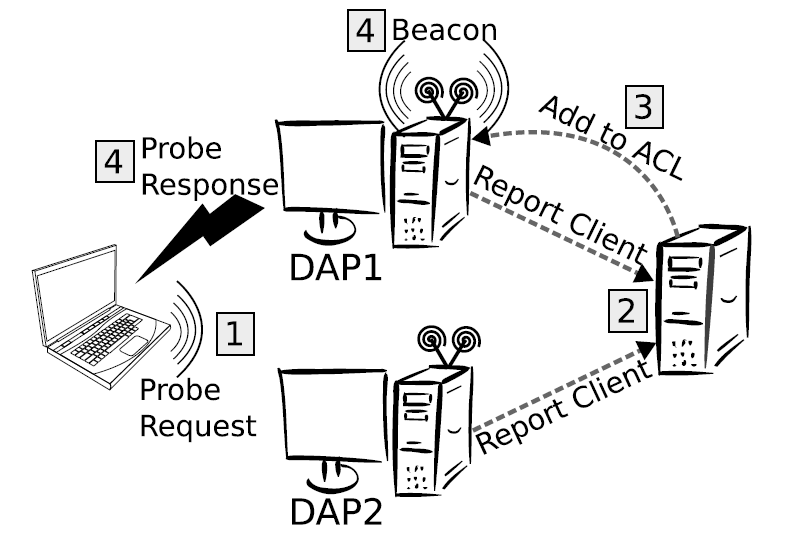
\includegraphics[scale=0.20]{img/fig2.png}
    \end{figure}
  \end{column}
  \end{columns}
\end{frame}
